\section{Methods}
The following methods come from \cite{luu}, in which a more detailed derivation can be found.
\subsection{Hubbard-Stratonovich Transformation}
Expectation values of operators can be calculated by the gaussian integral over quantum fields, as shown in \eqref{Pathintegral}. 
\begin{equation}\label{Pathintegral}
\langle O(t)\rangle = \frac{1}{Z} \operatorname{Tr}\left[O(t) e^{-\beta H}\right] =
\frac{1}{Z} \int\left[\prod_{i} d \psi_{i}^{\dagger} d \psi_{i}\right] e^{-\Sigma_{j}\left(\psi_{j}^{\dagger} \psi_{j}\right)}\bra{-\psi}O(t) e^{-\beta H}\ket{\psi}
\end{equation}
Here $Z $ is the partition function, which is defined as $Z:=\operatorname{Tr} \left[ e^{-\beta H}\right]$.
In the case of the Fermion-Hubbard-Model, these fields are fermion-fields, which anticommute with each other, therefore $\psi$ are Grassmann variables.
To solve $\bra{-\psi}O(t) e^{-\beta H}\ket{\psi}$, or just $\bra{-\psi}e^{-\beta H}\ket{\psi}$ for the partition function, one can cut the integral in infinitely many $(N_t\rightarrow\infty)$ time slices $\delta=\beta/N_t$ and introduce antiperiodic time boundaries $\psi_{N_t}=-\psi_{0}$, which is similar to the behavior of the thermal Green's function for fermions $G(\beta)=-G(0)$.
On these short time sections the Hamiltonian can be approximated (the larger $N_t$ is the more accurate), this approximation is relatively good for quadratic fields in the exponent, but the interaction term of the Hubbard-Model is quartic in the number of these fields.
%By slicing the integral into time sections it becomes a so called \emph{path integral}, which is commonly used in Quantum Field Theory.
The Hubbard-Stratonovich Transformation is basically a numerical trick to reduce the order of fermion fields. For $U\geq0$ we can linearize a quadradic term by introducing an auxiliary field, that we integrate over, as shown in \eqref{linearize}.
\begin{equation}\label{linearize}
e^{\frac{1}{2} U n^{2}}=\frac{1}{\sqrt{2 \pi U}} \int_{-\infty}^{\infty} d \phi\: e^{-\frac{1}{2 U} \phi^{2} \pm \phi n}
\end{equation}
Applying this to a time slice $\bra{\psi_{t+1}}e^{-\delta H} \ket{\psi_{t}}$ gives us for the Hubbard Hamiltonian with its diagonal interaction term
\begin{equation}\label{x}
\bra{\psi_{t+1}}e^{-\delta H} \ket{\psi_{t}}=\int_{-\infty}^{\infty}\left[\prod_{k} \frac{d \phi_{k}}{\sqrt{2 \pi\tilde{U}}}\right] e^{-\frac{1}{2 \tilde{U}} \phi^2}\bra{\psi_{t+1}}e^{-\sum_{j t} \tilde{t}_{j k} a_{j}^{\dagger} a_{k} \pm i \sum_{j} \phi_{j} n_{j}} \ket{\psi_{t}}
\end{equation}
where $\tilde{U}=\delta U$ and $\tilde{t}=\delta t$ are dimensionless parameters. 
Inserting this into the full path integral and writing all fermion operations as a matrix gives us \eqref{Z}
\begin{equation}\label{Z}
Z=\lim _{N_{t} \rightarrow \infty} \int_{-\infty}^{\infty} \mathcal{D}[\phi]e^{-\frac{1}{2 \tilde{U}} \phi^2}\int \mathcal{D}\left[\psi^{\dagger}, \psi\right] \exp \left\{-\sum_{i t^{\prime}, j t} \psi_{i t^{\prime}}^{\dagger} M[\phi]_{i t^{\prime}, j t} \psi_{j t}\right\}
\end{equation}
with the fermion matrix \eqref{M}
\begin{equation}\label{M}
M[\phi]_{i t^{\prime}, j t} \approx \delta_{i j} \delta_{t^{\prime} t}-e^{- \phi_{j, t}} \delta_{i j} \delta_{t^{\prime}, t+1}-\tilde{t} \delta_{< i,j>}\delta_{t^{\prime}, t+1}
\end{equation}
remember that due to our continuous time condition $\delta_{N_t,1}=-1$. The matrix form can be found in the appendix \ref{MM}. 
Performing the Gaussian integral in \eqref{Z} (with Grassmann variables!) results in these final equations (the second fermion matrix comes from the two spin degrees of freedom)
\begin{equation}\label{Zf}
Z=\lim _{N_{t} \rightarrow \infty} \int_{-\infty}^{\infty} \mathcal{D}[\phi]e^{-\frac{1}{2 \tilde{U}} \phi^2}\det(M[\phi]M[-\phi])
\end{equation}
\begin{equation}\label{Of}
\left\langle O\right\rangle =\lim _{N_{t} \rightarrow \infty} \int_{-\infty}^{\infty} \mathcal{D}[\phi]\:O[\phi]e^{-\frac{1}{2 \tilde{U}} \phi^2}\det(M[\phi]M[-\phi])
\end{equation}
The correlator $C_{\alpha\beta}(\tau) = \left\langle a_\alpha(\tau)a_\beta^\dagger(0)\right\rangle $, which is strongly connected to the fermion behavior and thus to the fermion matrix, can be calculated as follows
\begin{equation}\label{C}
C_{\alpha\beta}(\tau) =\lim _{N_{t} \rightarrow \infty} \int_{-\infty}^{\infty} \mathcal{D}[\phi]\:e^{-\frac{1}{2 \tilde{U}} \phi^2}M^{-1}_{\alpha\tau,\beta 0}[\phi]\det(M[\phi]M[-\phi])
\end{equation}

\subsection{Importance Sampling}
For the calculation of $Z$ and $C_{\alpha\beta}(\tau)$ integrals over the complete phase space $\phi$ have to be solved. Luckily the integrands can be disconnected into a normal distribution probability function (remember that $\sqrt{2\pi\tilde{U}}^{-1}$ is included in $\mathcal{D}[\phi]$) and the Matrix calculations.
Therefore instead of Monte Carlo integrating the whole integral, we sample $\phi$ by its importance from $\mathcal{N}_{0, \sqrt{\tilde{U}}}$ and calculate only the matrix part, which we then average.
For the one site Model the sampled $\phi$ lead to energy spectra of $M[\phi]$ that look like \ref{fig:spectra}.
\begin{figure}[H]
	\centering
	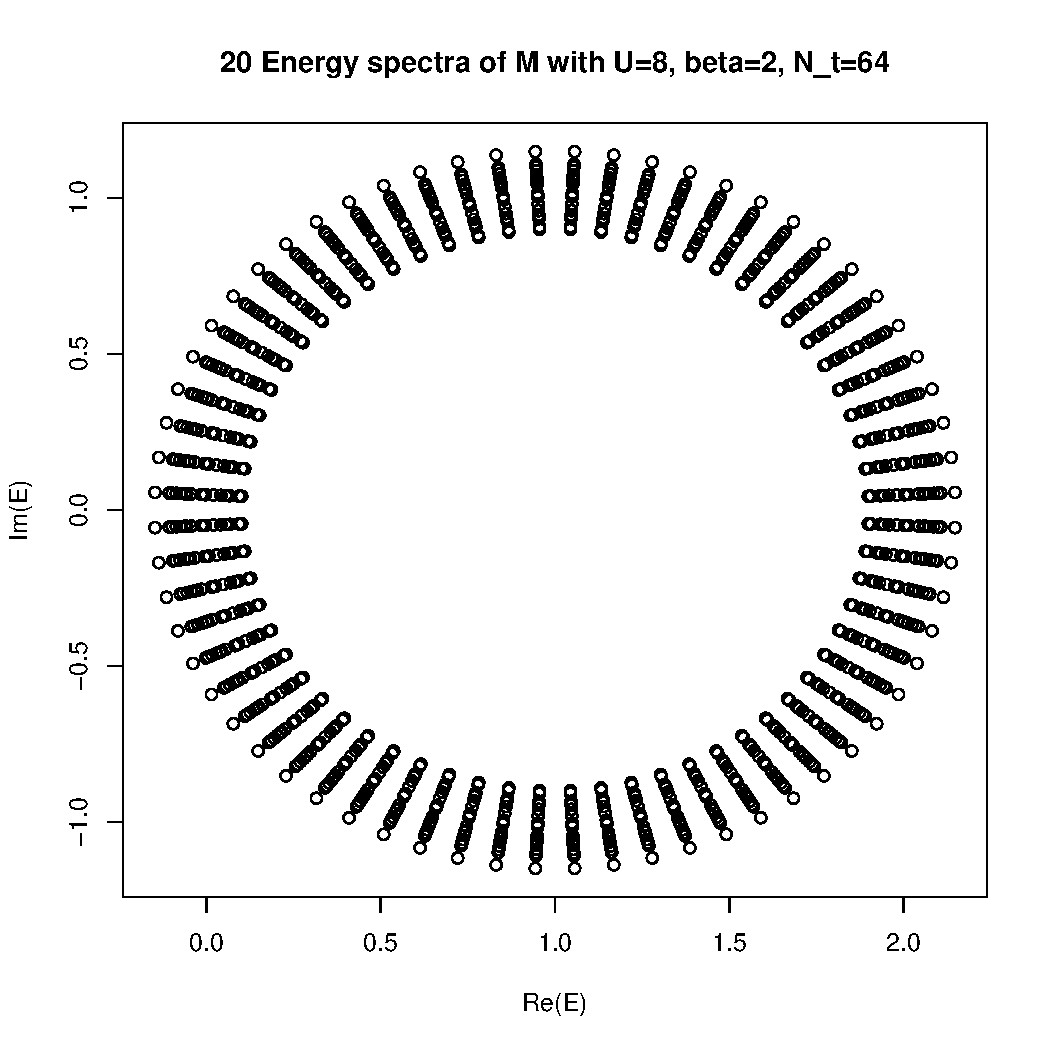
\includegraphics[width=0.5\linewidth]{figs/spectra}
	\caption[Energy Spectra]{Energy spectra for 20 sampled $\phi$, with $U=8$, $\beta=2$ and $N_t=64$}
	\label{fig:spectra}
\end{figure}
\begin{figure}[H]
	\centering
	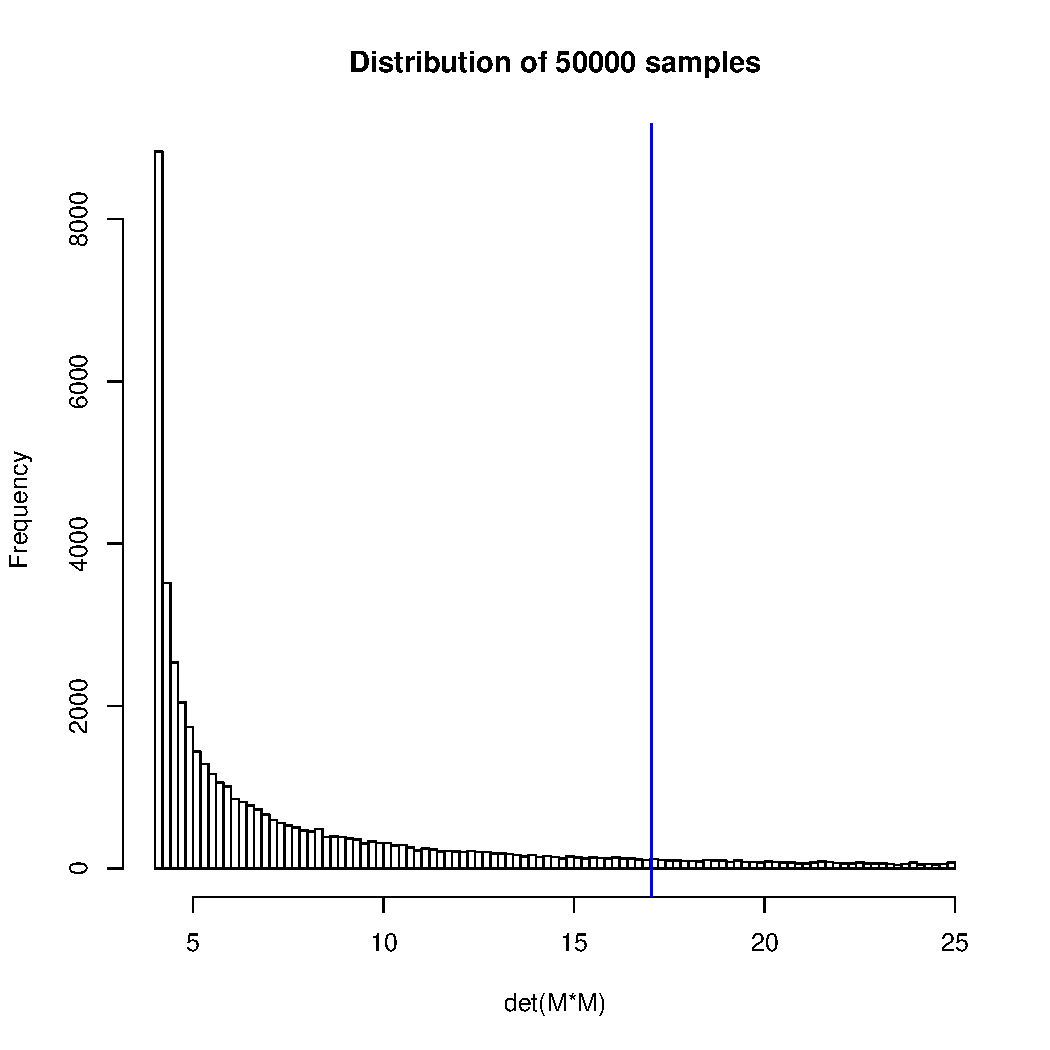
\includegraphics[width=0.5\linewidth]{figs/distribution}
	\caption[Distribution of 50000 samples]{This histogram shows the distribution of 50000 samples for a calculation of $Z$ for a 1 site lattice with $U=2$, $\beta=2$ and $N_t=24$. The blue line marks the mean, i.e. the result of the calculation. (Notice that the histogram was cut to focus on the interesting part)}
	\label{fig:distribution}
\end{figure}
Figure \ref{fig:distribution} shows how the sample calculations are distributed.